\newpage\subsection*{Άσκηση 3}

Κατασκευάστε ένα απλό συνεκτικό γράφο με 11 κορυφές και σύνολο βαθμών το \{3,4,5,8,10\}

\subsubsection*{Λύση}

Παρακάτω δίνονται οι γράφοι για τα σύνολα βαθμών $\{3,4,5,8,10\}, \{1,2,5\}$ αντίστοιχα. Οι γράφοι φτιάχτηκαν
μέσω της διαδικασίας που ακολουθήθηκε για την απόδειξη του θεωρήματος \en{Kapoor-Polimeni-Wall}.

\begin{center}
    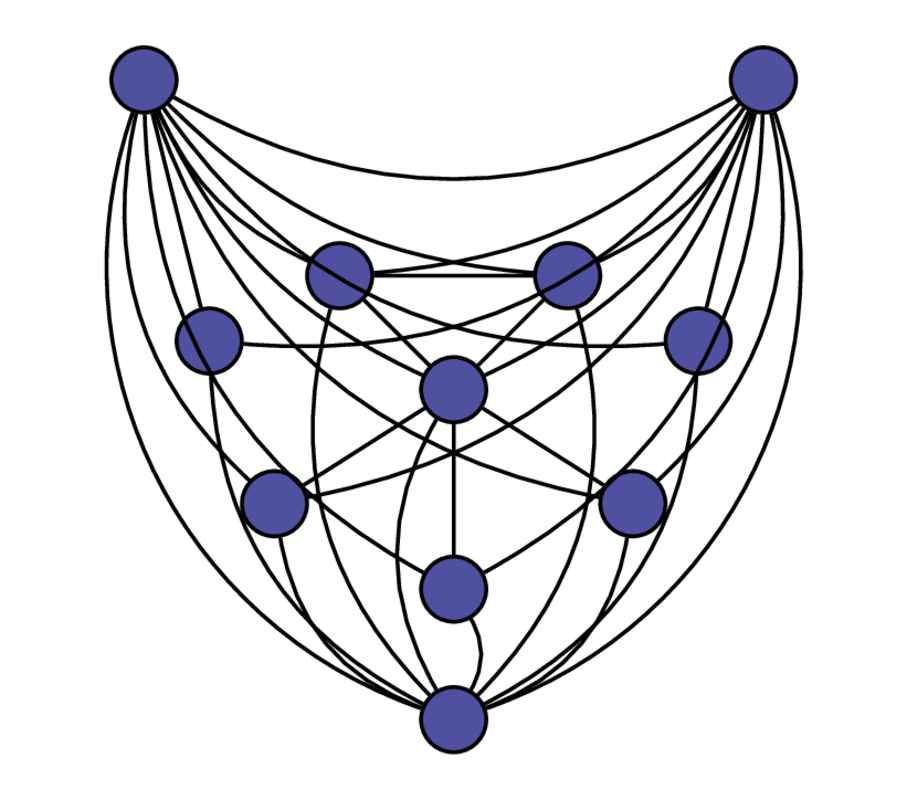
\includegraphics[width=.34\textwidth]{./exercise3/diagrams/d1.png} \hspace{3cm}
    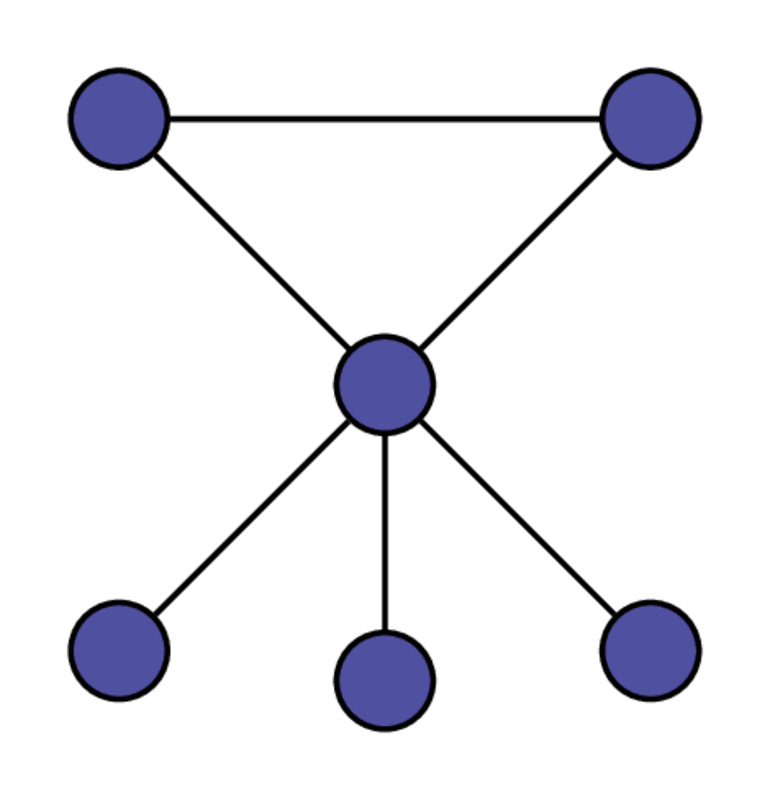
\includegraphics[height=5cm, width=.24\textwidth]{./exercise3/diagrams/d3.png}
\end{center}
